\documentclass[tikz]{standalone}
\usetikzlibrary{positioning,calc}

\begin{document}
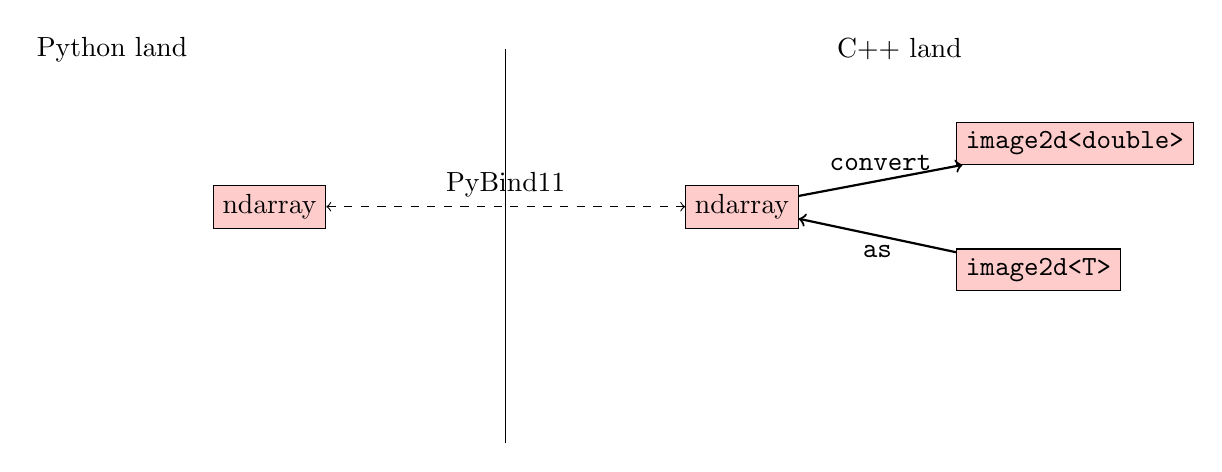
\begin{tikzpicture}
\tikzset{land/.style={draw}, obj/.style={draw,fill=red!20}};
   \draw node[] (A) {Python land} -- ++(10,0) node[] (B) {C++ land}; 
   \coordinate (C)  at ($(A)!0.5!(B)$);
   \draw (C) -- ++(0,-5);

   \node[obj] at (2,-2) (PyO) {ndarray};
   \node[obj] at (8,-2) (C) {ndarray};
   \node[obj] [above right=.25cm and 2cm of C] (D) {\tt image2d<double>};
   \node[obj] [below right=.25cm and 2cm of C] (E) {\tt image2d<T>};

   \draw[<->,dashed] (PyO) -- (C) node[midway,above] {PyBind11};
   \draw[->,thick] (C) -- (D)  node[midway,above]  {\tt convert};
   \draw[->,thick] (E) -- (C)  node[midway,below]  {\tt as};
   %%\draw[->] (D) -- (C) node[midway,above] {convert\_to};
 \end{tikzpicture}
 \end{document}